%\chapter{Preliminares. } % (fold)
Los proveedores de servicios de almacenamiento en la nube como lo son:  Dropbox, Mozy, Mega y otros, realizan la eliminación de archivos duplicados para ahorrar espacio en el servidor, almacenando sólo una copia de cada archivo cargado ~\ref{fig:4-0-1} \\
. Sin embargo, si los clientes cifran convencionalmente sus archivos es decir usando la criptografía simple (Simétrica y Asimétrica), se pierde ese ahorro de espacio. El cifrado de archivos con bloqueo de mensajes (conocido comunmente como el \textbf{Cifrado convergente} en adelante \textit{CE}) resuelve esta problemática. Sin embargo, está inherentemente sujeto a ataques de fuerza bruta que pueden recuperar archivos que caen en un conjunto conocido.\\


\begin{figure}[H]
\centering
	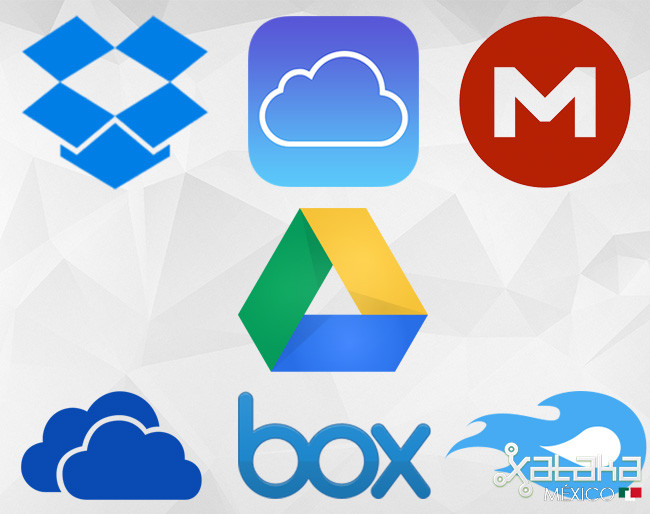
\includegraphics[width=7cm, height=4cm]{./images/servicios_nube.jpg}
	\caption{Servicios de almacenamiento en la nube}
	\label{fig:4-0-1}
\end{figure}

El protocolo criptográfico \textit{Dupless} propone una arquitectura que proporciona almacenamiento sin duplicaciones, seguro y resistente a ataques por fuerza bruta. En DupLESS, los clientes cifran sus archivos con claves basadas en mensajes obtenidas
desde un servidor de llaves a través de un protocolo OPRF inconsciente. Esto permite a los clientes almacenar datos cifrados con un servicio existente, y que este servicio realice la eliminación de duplicados en su nombre garantizando la confidencialidad. Dupless demuestra que el cifrado para el almacenamiento sin duplicados puede lograr ahorros de rendimiento y espacio cerca de utilizar el servicio de almacenamiento con datos de texto sin formato [].



\section{Diseño}

El protocolo criptográfico para la eliminación de duplicados DupLESS, esta diseñado e implementado para proporcionar una solución más segura y de fácil implementación para el cifrado de archivos que elimina la duplicación de estos. En DupLESS, los usuarios de este protocolo cifran sus archivos con la ayuda de un servidor de claves en adelante \textit{(KS)} que está separado del servicio de almacenamiento en adelante  \textit{Nube}. Los usuarios se autentican en el KS, pero no pierden la información sobre sus datos. Mientras que el KS permanezca inaccesible para los atacantes, el protocolo puede garantizar una alta seguridad (Seguridad semántica). Si en algún momento el KS y la Nube están comprometidos, Dupless conserva la actual garantía MLE de seguridad para mensajes impredecibles.\\ 

El principal objetivo de DupLESS, es hacer que dicho protocolo trabaje de forma transparente con los sistemas en la Nube que hasta ahora se encuentran en funcionamiento, por lo que DupLESS funciona como una capa sobre las interfaces de almacenamiento simples que acceden a la Nube. Esto también significa que DupLESS es desarrollado: para ser lo más incompatible posible con los comandos existentes en las API's de estos sistemas en la Nube exixtentes, para que así no se tenga ningún conocimiento sobre los sistemas que implementan estas API, para dar un rendimiento muy cercano al de usar la Nube sin ningún cifrado, y lograr el mismo nivel de disponibilidad que el proporcionado por la Nube.


\section{Funcionamiento}

DupLESS contempla que un atque por fuerza bruta a un texto cifrado dentro de un esquema de tipo CE puede tratarse utilizando un servidor de llaves (KS) para derivar llaves a partir de un archivo, en lugar de establecer llaves con funciones hash de los archivos. Para poder acceder al KS, se debe de realizar el procedimiento de autenticación a los usuarios del protocolo, esto detiene a los atacantes externos. El aumento de los costos a los ataques, disminuye los ataques por fuerza bruta hacia los usuarios comprometidos y ahora el KS puede funcionar como un único punto de control para implementar medidas de limitación de velocidad. \\

Para poder implementar un esquema seguro y que evite la duplicación de archivos, Dupless crea un servidor de llaves KS el cuál proveera de llaves para el cifrado de un archivo, dicho servidor se comunica con el cliente a través de un protocolo llamado OPRF,este protocolo proveerá de algoritmos para la autenticación de usuarios y el cifrado convergente de los archivos que se van a almacenar, dicho protocolo funciona de la siguiente manera: \\ 

\textbf{OPRF} es un esquema que consta de cinco algoritmos (Kg, EvC, EvS, Vf, Ev), los últimos dos deterministas. 

\begin{itemize}
	\item \textit{Generación de claves Kg: } \\
	 (pk, sk) \$ ← Kg. Este algoritmo genera una llave pública \textit{pk} que puede distribuirse libremente entre varios usuarios, y una clave secreta \textit{sk}, que permanece solo en el servidor de llaves. Dichas claves serán parte del servidor, son generadas a través de la criptografía asimétrica usando el algoritmo RSA.


	\item \textit{EvC: }\\ 
	La evaluación de este protocolo comienza del lado del cliente: 
	\begin {enumerate}
		\item Se obtiene del servidor la llave pública \textit{e} y se realiza una comparación con  \textit{e $\leq$ N}, N fue el producto de 2 números primos utilizado en la generación de llaves del servidor. Si la comparación no se cumple, el protocolo envía un error.
		\item Se elige un número aleatorio dentro del campo de los números < N. 
		\item Se realiza una función hash al archivo que se desea cargar a la Nube, almacenandola en la variable\textit{h ← H(M)} 
		\item Ahora se multiplica la función hash del mensaje por el número aleatorio elevado a la llave pública del servidor\textit{r$^e$} y se almacena en \textbf{\textit{x}}  \hspace{2cm} \textit{x ← h $\cdot$ r$^e$ mod N}
		\item Esta \textbf{\textit{x}} es enviada al servidor de llaves, en donde será firmada por este sin saber su contenido ni procedencia, es decir para realizar una firma a ciegas del mensaje a cargar. 
		\item La firma por el servidor es recibida al cliente y se realiza la siguiente operación  \hspace{2cm} \textit{z ← y $\cdot$ r$^-1$ mod N}

.
\end{enumerate}
\item \textit{EvS: }\\ 
        Del lado del servidor, se recibe la entrada \textit{x} que corresponde a la función hash del archivo enviada por el lado del cliente. El servidor sólo realiza una operación la cuál es la firma con la llave privada del servidor. Dicha firma, es a ciegas ya que el servidor no conoce el contenido del archivo ni la procedencia de quien lo esta enviando. Dicha firma se realiza de la siguiente manera:    \hspace{2cm} \textit{y ← x$^d$ mod N}






\end{itemize}





